\documentclass[a4paper, 12pt]{article}
\usepackage[T2A,T1]{fontenc}
\usepackage[utf8]{inputenc}
\usepackage[english, ukrainian]{babel}
\usepackage{amsmath}
\usepackage{amssymb}
\usepackage{mathtools}
\usepackage{euler}
% \usepackage[dvipsnames]{xcolor}
\usepackage{xcolor}
\usepackage[margin=1.5cm]{geometry}
\usepackage{float}
\usepackage{multirow}
\usepackage{multicol}
\usepackage{url}
\usepackage[unicode=true, colorlinks=true, linktoc=all, linkcolor=blue]{hyperref}
\usepackage{cite}
\usepackage{amsthm}
\usepackage{thmtools}
\usepackage[framemethod=TikZ]{mdframed}
\usepackage[toc,page,title,titletoc]{appendix}
\usepackage{bookmark}
\usepackage[nottoc,notlot,notlof]{tocbibind}
\usepackage{minted}
% \usepackage[hang]{footmisc}
\theoremstyle{definition}
\mdfdefinestyle{mdbluebox}{%
	roundcorner = 10pt,
	linewidth=1pt,
	skipabove=12pt,
	innerbottommargin=9pt,
	skipbelow=2pt,
	nobreak=true,
	linecolor=blue,
	backgroundcolor=TealBlue!5,
}
\declaretheoremstyle[
	headfont=\sffamily\bfseries\color{MidnightBlue},
	mdframed={style=mdbluebox},
	headpunct={\\[3pt]},
	postheadspace={0pt}
]{thmbluebox}

\mdfdefinestyle{mdredbox}{%
	linewidth=0.5pt,
	skipabove=12pt,
	frametitleaboveskip=5pt,
	frametitlebelowskip=0pt,
	skipbelow=2pt,
	frametitlefont=\bfseries,
	innertopmargin=4pt,
	innerbottommargin=8pt,
	nobreak=true,
	linecolor=RawSienna,
	backgroundcolor=Salmon!5,
}
\declaretheoremstyle[
	headfont=\bfseries\color{RawSienna},
	mdframed={style=mdredbox},
	headpunct={\\[3pt]},
	postheadspace={0pt},
]{thmredbox}

\declaretheorem[style=thmbluebox,name=Теорема,numberwithin=section]{theorem}
\declaretheorem[style=thmbluebox,name=Теорема,numbered=no]{theorem*}
\declaretheorem[style=thmbluebox,name=Лема,sibling=theorem]{lemma}
\declaretheorem[style=thmbluebox,name=Лема,numbered=no]{lemma*}
\declaretheorem[style=thmbluebox,name=Твердження,sibling=theorem]{proposition}
\declaretheorem[style=thmbluebox,name=Наслідок,sibling=theorem]{corollary}
\declaretheorem[style=thmredbox,name=Приклад,sibling=theorem]{example}

\mdfdefinestyle{mdgreenbox}{%
	skipabove=8pt,
	linewidth=2pt,
	rightline=false,
	leftline=true,
	topline=false,
	bottomline=false,
	linecolor=ForestGreen,
	backgroundcolor=ForestGreen!5,
}
\declaretheoremstyle[
	headfont=\bfseries\sffamily\color{ForestGreen!70!black},
	bodyfont=\normalfont,
	spaceabove=2pt,
	spacebelow=1pt,
	mdframed={style=mdgreenbox},
	headpunct={ --- },
]{thmgreenbox}

\mdfdefinestyle{mdblackbox}{%
	skipabove=8pt,
	linewidth=3pt,
	rightline=false,
	leftline=true,
	topline=false,
	bottomline=false,
	linecolor=black,
	backgroundcolor=RedViolet!5!gray!5,
}
\declaretheoremstyle[
	headfont=\bfseries,
	bodyfont=\normalfont\small,
	spaceabove=0pt,
	spacebelow=0pt,
	mdframed={style=mdblackbox}
]{thmblackbox}

% \theoremstyle{theorem}
\declaretheorem[name=Запитання,sibling=theorem,style=thmblackbox]{ques}
\declaretheorem[name=Вправа,sibling=theorem,style=thmblackbox]{exercise}
\declaretheorem[name=Зауваження,sibling=theorem,style=thmgreenbox]{remark}
\declaretheorem[name=Припущення,sibling=theorem,style=thmblackbox]{assumption}

\theoremstyle{definition}
\newtheorem{claim}[theorem]{Твердження}
\newtheorem{definition}[theorem]{Визначення}
\newtheorem{fact}[theorem]{Факт}

\newtheorem{problem}{Задача}[section]
\newtheorem{sproblem}[problem]{Задача}
\newtheorem{dproblem}[problem]{Задача}
\renewcommand{\thesproblem}{\theproblem$^{\star}$}
\renewcommand{\thedproblem}{\theproblem$^{\dagger}$}

\makeatletter
\newenvironment{solution}[1][\solutionname]{\par
  \pushQED{\qed}%
  \normalfont \topsep6\p@\@plus6\p@\relax
  \trivlist
%<amsbook|amsproc>  \itemindent\normalparindent
  \item[\hskip\labelsep
%<amsbook|amsproc>        \scshape
%<amsart|amsthm>        \itshape
\itshape 
    #1\@addpunct{.}]\ignorespaces
}{%
  \popQED\endtrivlist\@endpefalse
}
%    \end{macrocode}
%    Default for \cn{proofname}:
%    \begin{macrocode}
\providecommand{\solutionname}{Розв'язок}

\makeatother
\renewcommand{\phi}{\varphi}
\renewcommand{\epsilon}{\varepsilon}

\newcommand{\NN}{\mathbb{N}}
\newcommand{\ZZ}{\mathbb{Z}}
\newcommand{\QQ}{\mathbb{Q}}
\newcommand{\RR}{\mathbb{R}}
\newcommand{\CC}{\mathbb{C}}

\newcommand{\la}{\mathcal{L}}
\newcommand{\ca}{\mathcal{C}}
\newcommand{\hi}{\mathcal{H}}

\newcommand{\no}[1]{\left\| #1 \right\|}
\renewcommand{\sp}[1]{\left\langle #1 \right\rangle}
% \renewcommand{\sp}[2]{\left\langle #1, #2 \right\rangle}
\renewcommand{\bar}{\overline}

\newcommand*\diff{\mathop{}\!\mathrm{d}}
\newcommand*\rfrac[2]{{}^{#1}\!/_{\!#2}}

\DeclareMathOperator{\argmin}{argmin}
\DeclareMathOperator{\epigraph}{epi}
\DeclareMathOperator{\proximal}{prox}
\DeclareMathOperator{\diagonal}{diag}
\DeclareMathOperator{\domain}{dom}
\DeclareMathOperator{\trace}{tr}

\DeclareMathOperator*{\Argmin}{argmin}
\DeclareMathOperator*{\Min}{min}
\DeclareMathOperator*{\Inf}{inf}
\DeclareMathOperator*{\Sup}{sup}
\DeclareMathOperator*{\Lim}{lim}

\DeclareMathOperator*{\Sum}{\sum}
\DeclareMathOperator*{\Int}{\int}

\renewcommand{\appendixtocname}{Додаток}
\renewcommand{\appendixpagename}{Додаток}
\renewcommand{\appendixname}{Додаток}
\makeatletter
\let\oriAlph\Alph
\let\orialph\alph
\renewcommand{\@resets@pp}{\par
  \@ppsavesec
  \stepcounter{@pps}
  \setcounter{section}{0}%
  \if@chapter@pp
    \setcounter{chapter}{0}%
    \renewcommand\@chapapp{\appendixname}%
    \renewcommand\thechapter{\@Alph\c@chapter}%
  \else
    \setcounter{subsection}{0}%
    \renewcommand\thesection{\@Alph\c@section}%
  \fi
  \if@pphyper
    \if@chapter@pp
      \renewcommand{\theHchapter}{\theH@pps.\oriAlph{chapter}}%
    \else
      \renewcommand{\theHsection}{\theH@pps.\oriAlph{section}}%
    \fi
    \def\Hy@chapapp{appendix}%
  \fi
  \restoreapp
}
\makeatother

\renewcommand\thempfootnote{\alph{mpfootnote}}
\newcommand{\todo}[1]{\footnote{\textcolor{red}{TODO}: #1}}

\newcommand{\cover}[2]{
\begin{center}
\hfill \break \bf
  М{\smallІНІСТЕРСТВО ОСВІТИ ТА НАУКИ} У{\smallКРАЇНИ} \\
  К{\smallИЇВСЬКИЙ НАЦІОНАЛЬНИЙ УНІВЕРСИТЕТ ІМЕНІ} Т{\smallАРАСА} Ш{\smallЕВЧЕНКА} \\ 
  Ф{\smallАКУЛЬТЕТ КОМП'ЮТЕРНИХ НАУК ТА КІБЕРНЕТИКИ} \\
  К{\smallАФЕДРА ОБЧИСЛЮВАЛЬНОЇ МАТЕМАТИКИ}
\end{center}

\vfill 

\begin{center}
  \LARGE \bf
  Звіт до лабораторної роботи №{#1} на тему \\ 
  \guillemotleft{#2}\guillemotright
\end{center}

\vfill 

\begin{flushright}
  \large \bf 
  Виконав студент групи ОМ-3 \\
  
  Скибицький Нікіта
\end{flushright}

\vfill 

\begin{center}
  \large \bf
  Київ --- 2019
\end{center}

\thispagestyle{empty} 
\newpage
}
\newcommand{\people}{
    У виконанні роботи брали участь:
    \begin{itemize}
        \item Основні учасники:
        \begin{itemize}
            \item Скибицький Нікіта
            \item Сергієнко Тетяна
            \item Тихонравова Юлія
            \item Ковальчук Віктор
            \item Кузьмінова Катерина 
            \item Антипова Аліса
        \end{itemize}
        \item Також допомагали:
        \begin{itemize}
            \item Пушкін Денис
            \item Єрмаков Артур
            \item Бельо Андрій
            \item Гронь Ілля
        \end{itemize}
    \end{itemize}
    \newpage
}

\author{Скибицький Нікіта}
\date{\today}

\allowdisplaybreaks
\numberwithin{equation}{section}
\linespread{1.15}

\begin{document}

\cover{3}{Мурашиний алгоритм}

\people

\tableofcontents

\section{Постановка задачі}

Задано орієнтований граф $G = (V, E)$. Ребро $e_i \in E$ графа характеризуються довжиною $\ell_i$. Задано початкову вершину $s \in V$ і цільову (кінцеву, фінальну) вершину $f \in V$. \medskip

Необхідно знайти найкоротший шлях із $s$ до $f$.

\section{Неформальний опис алгоритму}

Розглянемо популяцію з $N$ мурах, які протягом $M$ ітерацій намагаються знайти найкоротший шлях (наприклад, шлях доставки листя до мурашника). \medskip

Уявімо, що на кожній ітерації кожна мурашка проходить якийсь шлях, залишаючи на своєму шляху феромени, і керуючись вже наявними із попередніх ітерацій фероменами для вибору шляху.

\section{Код програмного продукнту}

\subsection{Представлення графу у пам'яті програми}

\inputminted[firstline=64, lastline=75]{python}{../../code/salesman/main.py}

де ребро моделюєтсья наступним класом:

\inputminted[firstline=55, lastline=60]{python}{../../code/salesman/main.py}

Як бачимо, у ребра є довжина (\verb|length|), на ньому є певна інтенсивність фероменів (\verb|feroment|), і необхідне оновлення фероментів (\verb|delta|).

\subsection{Клас, який моделює мурашку}

\subsubsection{Конструктор}

\inputminted[firstline=6, lastline=13]{python}{../../code/salesman/main.py}

Як ми бачимо з коду, кожна мурашка пам'ятає список вже пройдених вершин (\verb|tabu_list|), знає у якій вершині вона зараз знаходиться (\verb|vertice|), знає, куди їй треба йти (\verb|target|), підтримує у пам'яті загальну довжину пройденого шляху (\verb|path_length|), сам цей шлях (\verb|path|) і знає, чи вона ``жива'' (\verb|alive|). \textit{Мурашка вважається ``мертвою'', якщо вона не змогла дістатися мурашника.}

\subsubsection{Метод для вибору напрямку кроку}

\inputminted[firstline=15, lastline=44]{python}{../../code/salesman/main.py}

\subsubsection{Метод для пошуку цілісного шляху:}

\inputminted[firstline=46, lastline=52]{python}{../../code/salesman/main.py}

\subsection{Програма-драйвер}

\inputminted[firstline=82, lastline=91]{python}{../../code/salesman/main.py}

\section{Тестування програмного продукту}

\subsection{Граф}

Ось так виглядає наш тестовий граф:
\begin{figure}[H]
    \centering
    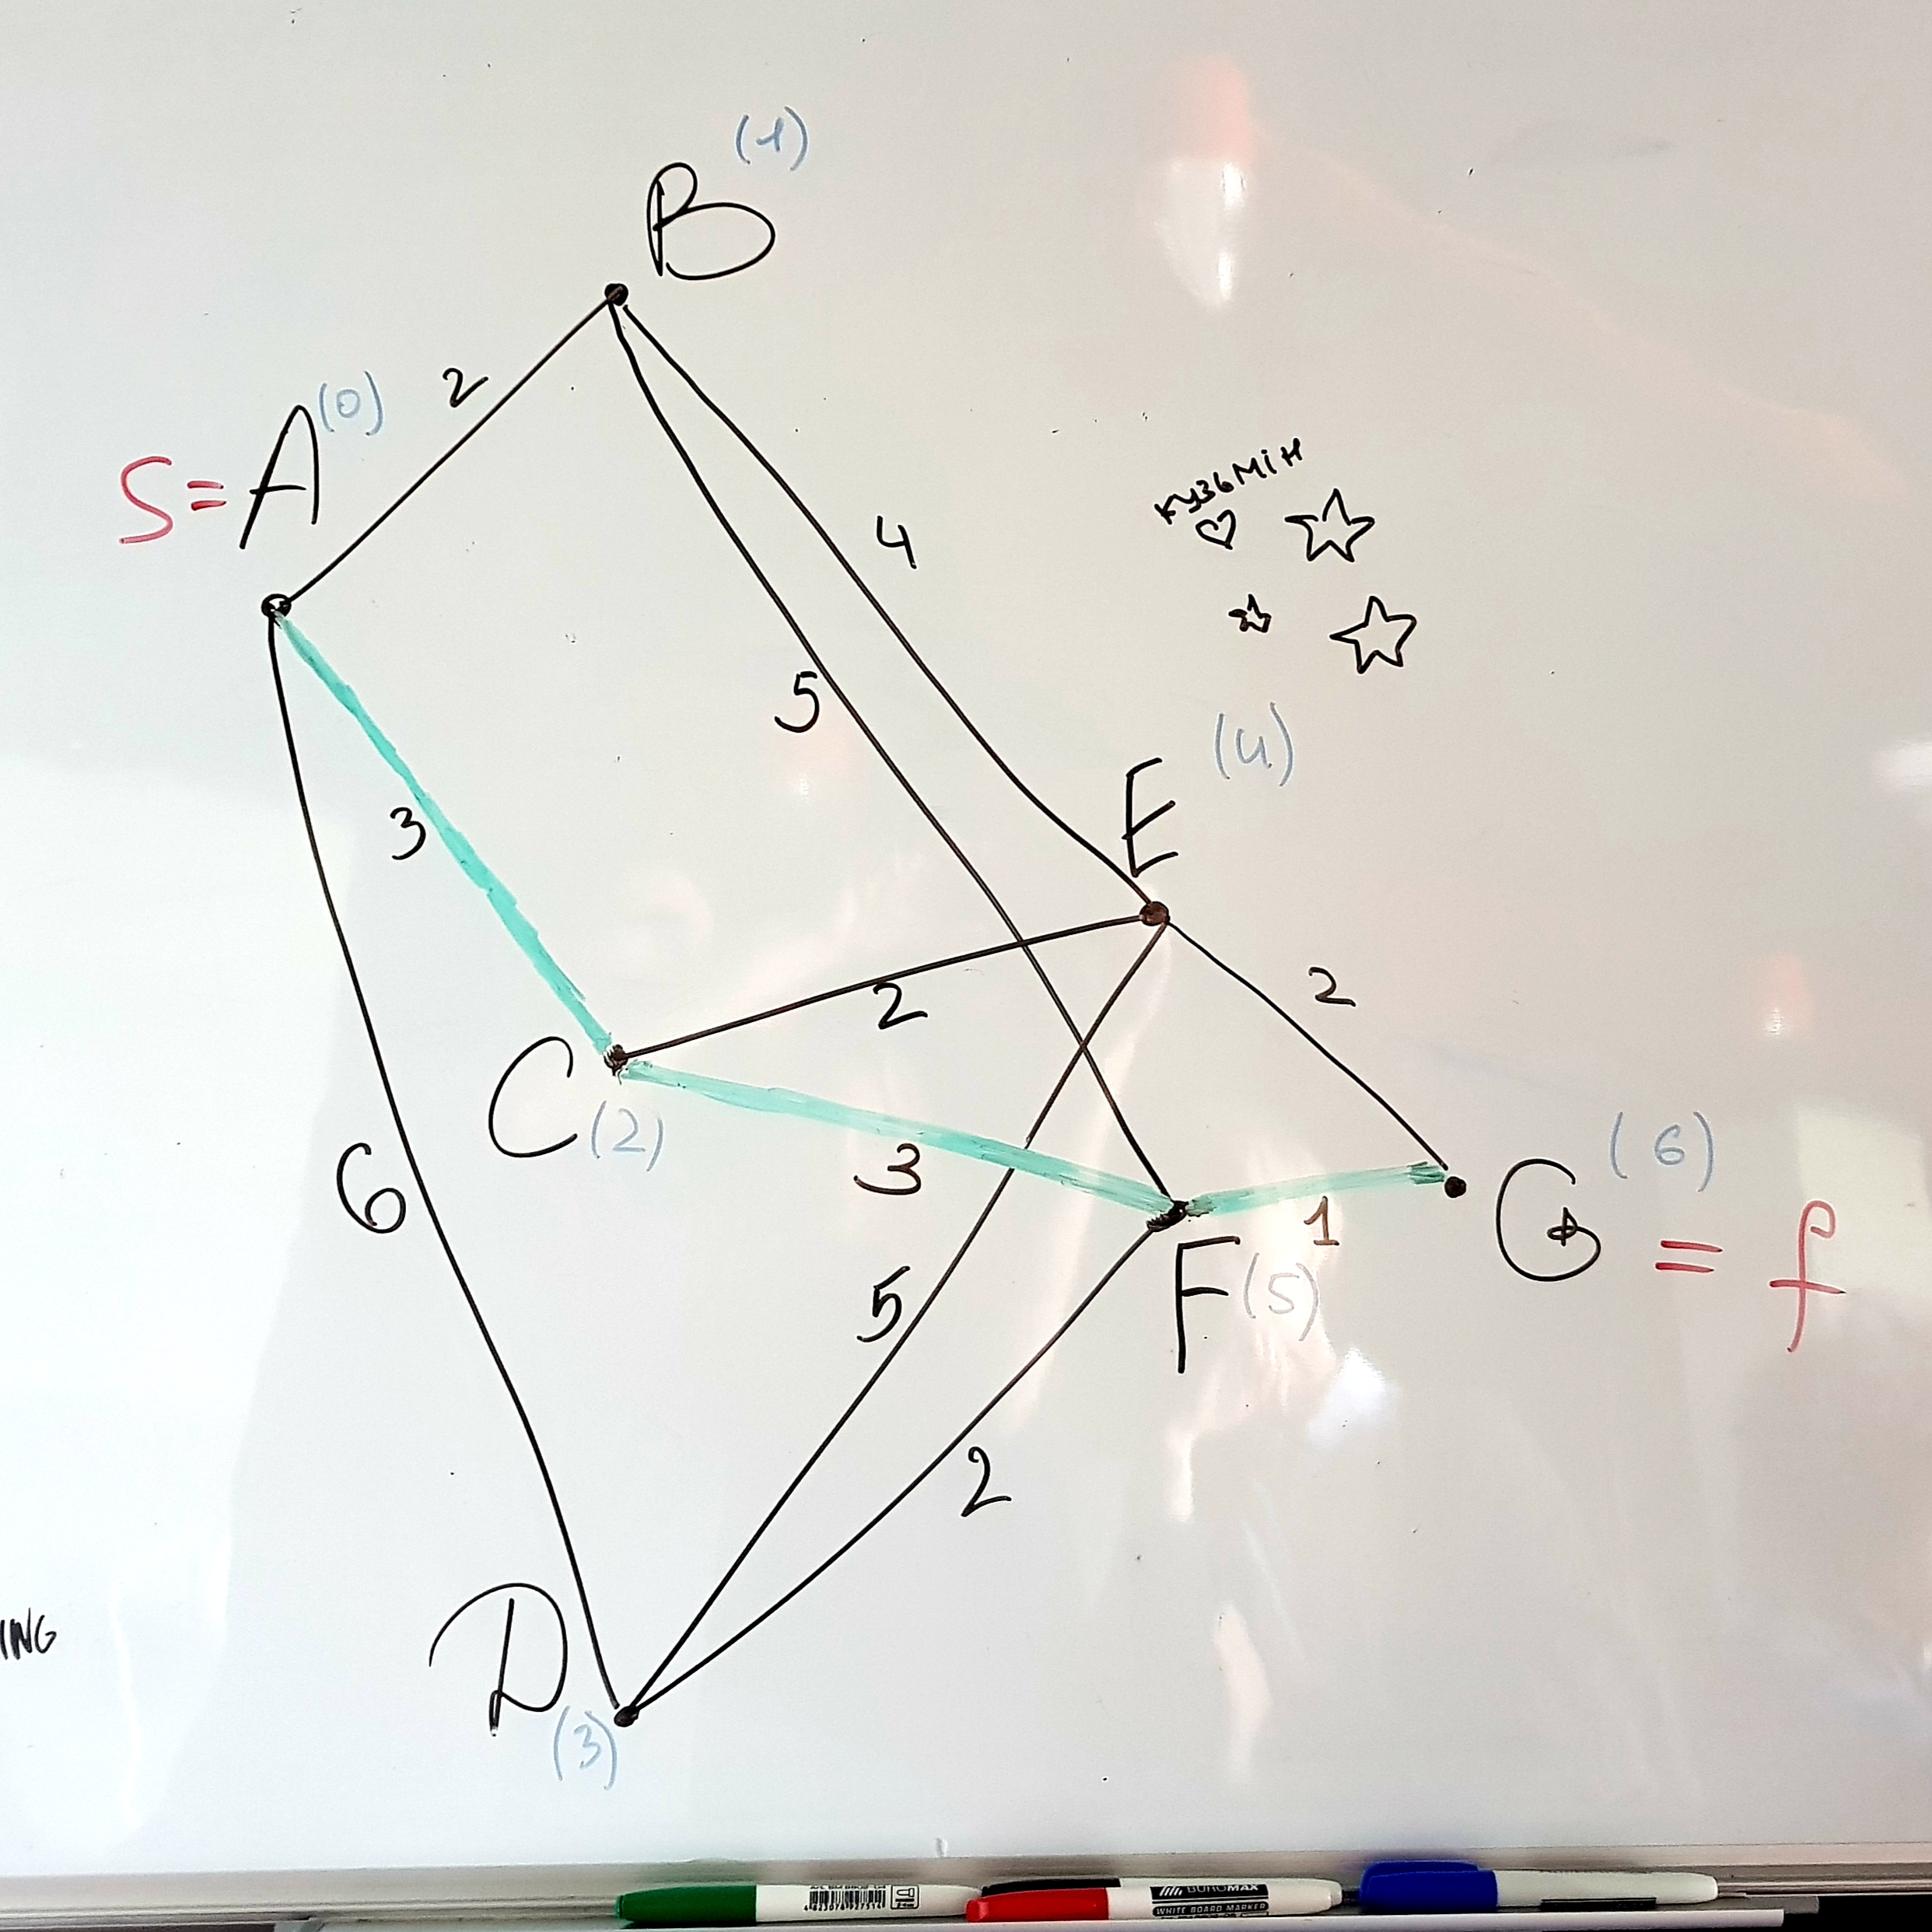
\includegraphics[width=\textwidth]{../../code/salesman/graph.jpg}
\end{figure}

\subsection{Графіки}

Інтенсивність фероменів від ітерації:

\subsubsection{10 ітерацій}

\begin{figure}[H]
    \centering
    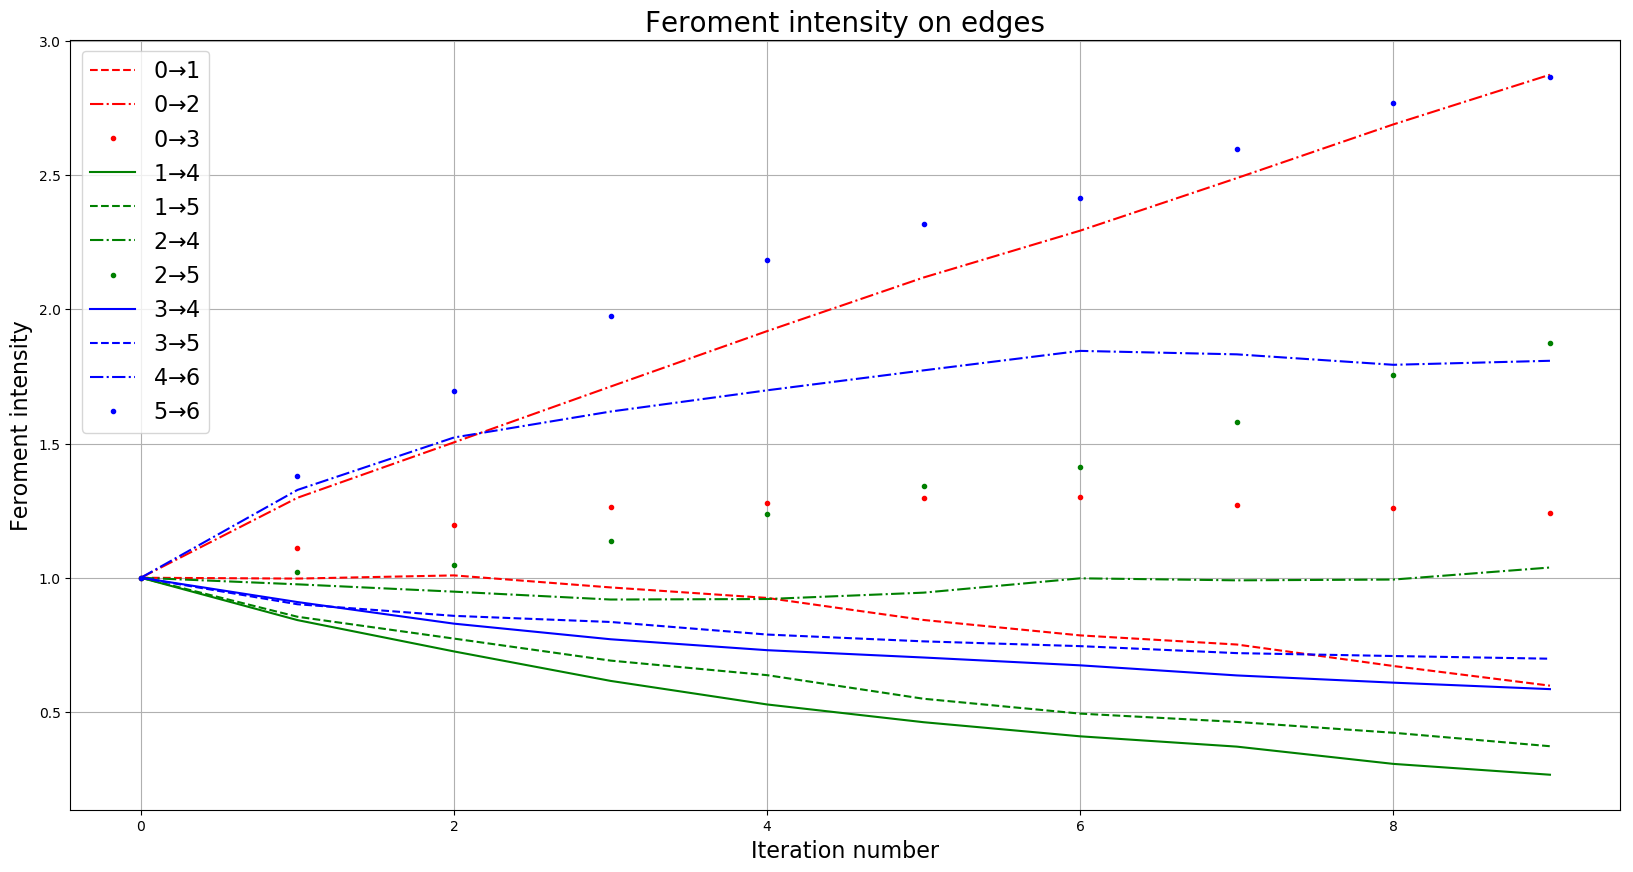
\includegraphics[width=\textwidth]{../../code/salesman/feroment_10.png}
\end{figure}

\subsubsection{100 ітерацій}

\begin{figure}[H]
    \centering
    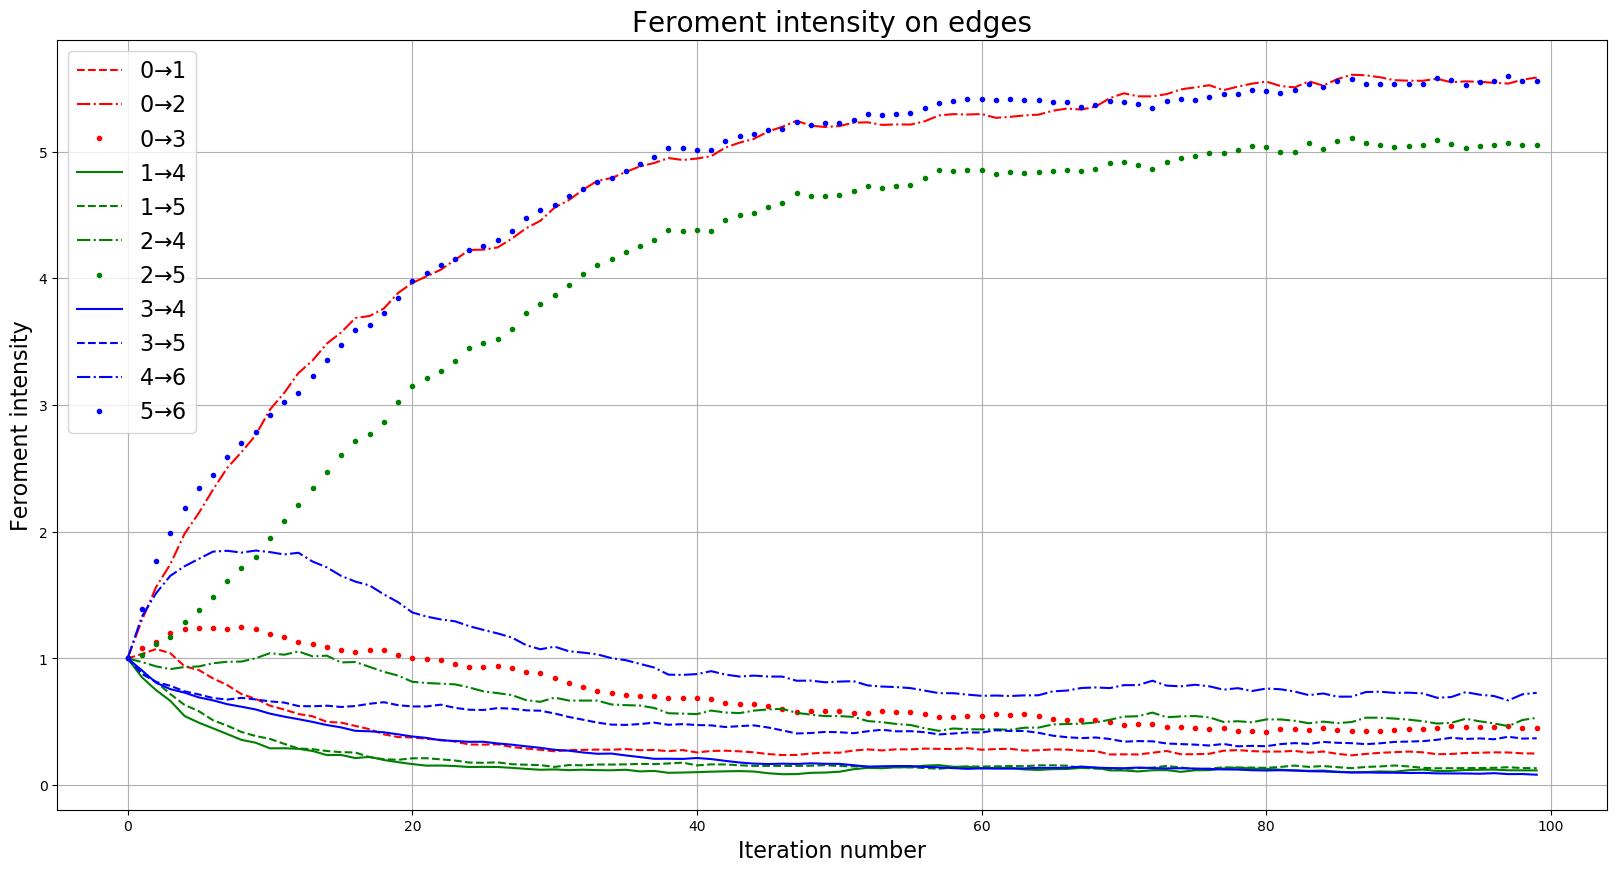
\includegraphics[width=\textwidth]{../../code/salesman/feroment_100.png}
\end{figure}

\subsubsection{1000 ітерацій}

\begin{figure}[H]
    \centering
    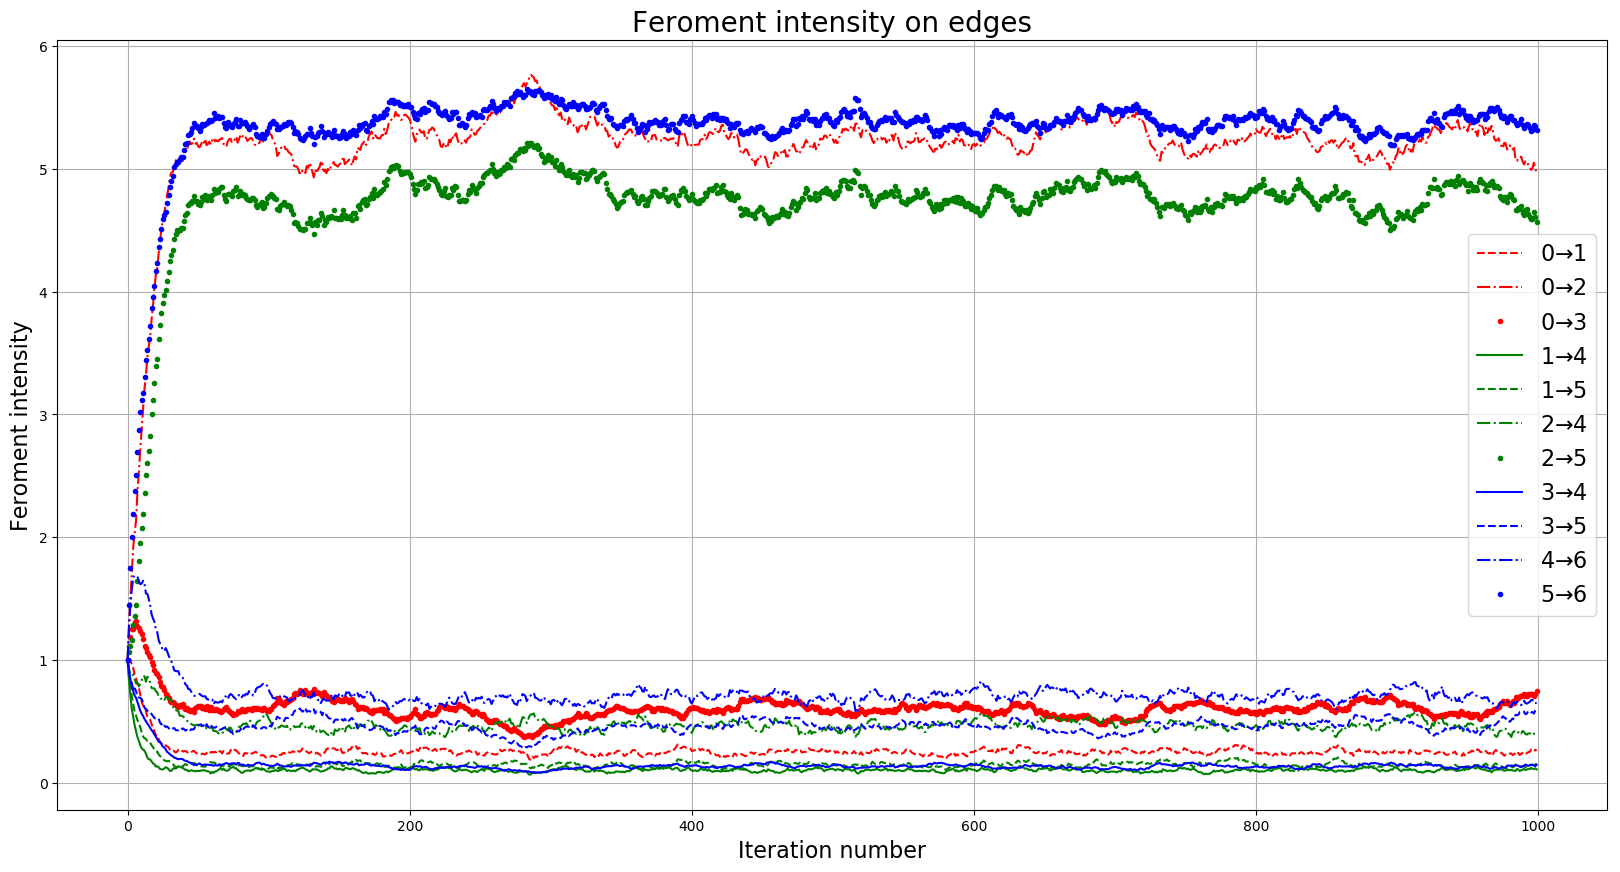
\includegraphics[width=\textwidth]{../../code/salesman/feroment_1000.png}
\end{figure}

\subsection{Швидкодія}

Середній час виконання ітерації --- \textbf{0.179} секунди, або \textbf{3} хвилини на \textbf{1000} ітерацій. \medskip

Зауважимо, що алгоритм багатоагентний і ідеально паралелиться, тому насправді нас цікавить час виконання однією мурахою однієї ітерації.  \medskip

Нескладно зрозуміти, що час виконання однієї мурахо-ітерації мізерний, а саме \textbf{0.000179} секунди, тобто одна мурашка може виконати понад \textbf{5000} ітерацій за одну секунду. \medskip

На більшому графі ($\vert V \vert = 30$, $\vert E \vert = 100$) швидкодія передбачувано знизиться, але все одно складе принаймні \textbf{100} ітерацій на секунду. \medskip

Тобто, маючи \textbf{16} логічних процесорів (а саме стільки їх у моєму ноутбуці) і розпаралеливши алгоритм можна розв'язати у \textbf{50} разів складнішу (і вже цілком реалістичну) задачу десь за \textbf{30} хвилин. \medskip

Непоганий результат, враховуючи що сама постановка задачі NP-повна.

% \newpage
% \bibliography{main}
% \bibliographystyle{ieeetr}

\end{document}